\documentclass[a4paper,10pt]{report}
\usepackage[brazil]{babel}
\usepackage[utf8]{inputenc}

\usepackage[pdftex]{graphicx}
\usepackage{caption}
\usepackage{subcaption}
\usepackage{amssymb}
\usepackage{amsmath}

% \hyphenation{}

\usepackage[pdftex]{hyperref}
\hypersetup{
    pdfborder = {0 0 0}
}
\usepackage[alf,abnt-etal-cite=2,abnt-etal-list=0,abnt-etal-text=emph]{abntex2cite}

%opening
\author{Ricardo Bustamante de Queiroz}
\title{Tópicos Especiais em Computação Gráfica\\-- Artigos --}


\begin{document}

\maketitle
\tableofcontents

\chapter{Mês de agosto}
%\input{artigos/1998_Atluri_ComputationalMechanics_MeshlessPetrovGalerkinComputMechanics/report_1998_atluri}
\section{\textit{Synthesizing Parameterized Motions}}

% ============================================================================
\subsection{Referência completa do artigo}

\begin{itemize}
  \item \textbf{Autores:} Michiel van de Panne, Ryan Kim, Eugene Fiume
  \item \textbf{Local:} University of Toronto
  \item \textbf{\textit{Journal}:} Eurographics
Workshop on Animation and Simulation [Qualis : não encontrei]
  \item \textbf{Data:} Sept. 17-18, 1994
  \item \textbf{Referência:} \citeonline{bib:1994:synthesizing}
\end{itemize}


% ============================================================================
\subsection{Resumo}

%Máquinas de estado finito são utilizadas para alternar entre parâmetros de controle, para permitir movimentações cíclicas mais complexas, e decisões de novas poses podem ser tomadas baseadas em dados obtidos por sensores.
\subsubsection{Abstract}

In striving to construct higher level control representations for simulated characters or creatures, one must seek flexible control representations to build upon. We present a method for the synthesis of parametrized, physics-based motions. The method can be applied to both periodic and aperiodic motions. The basis of the method is a low-level control representation in which linear combinations of controllers generally produce predictable in-between motions.

% ..........................................................
\subsubsection{Propósito do artigo}

O artigo propõe um método de gerar movimentos realisticos de forma reusável e parametrizada, isto é, evitando que o problema de controle tenha de ser resolvido novamente para cada novo caso específico.

Existem diversas técnicas de animação para gerar tais movimentos. O autor optou pelo uso de controladores, onde há uma informação de como o movimento deve ser realizado, mas respeitando restrições como a física, causando um aumento de realidade na ação. 

Um controlador pode ser tornado mais versátil adicionando a capacidade de parametrização de seus atributos, e podem receber informação do ambiente, permitindo reações a estímulos externos durante a movimentação.

% ..........................................................
\subsubsection{Técnicas utilizadas} 
\begin{itemize}
  \item Controladores PD
  \item Máquinas de estado finito
  \item Algoritmos Genéticos
  \item Otimização em duas fases
  \item Arrefecimento simulado
  \item Método do gradiente
\end{itemize}  

% ..........................................................
\subsubsection{Contribuição em relação a artigos anteriores} %mais ou menos 10 linhas
 \begin{itemize}
   \item Um estudo anterior havia sido feito para casos em que a movimentação era exclusivamente cíclica. O artigo expande essa noção para aplicar a qualquer topologia de grafo de pose.
   \item O poder computacional necessário para sintetizar uma solução foi drasticamente reduzido em relação a mais de uma solução anterior.
 \end{itemize}  

% ============================================================================
\subsection{Metodologia}
% Descreva um pouco mais detalhadamente a metodologia e os resultados do artigo. 
% Inclua as figuras que achar mais relevantes.

\subsubsection{Grafos de controle de pose}

Máquinas de estado finito são utilizadas para alternar entre parâmetros de controle, para permitir movimentações cíclicas mais complexas. Decisões de novas poses também podem ser tomadas baseadas em dados obtidos por sensores.

Uma pose é definida por um conjunto de graus de liberdade do modelo.

%A figura \ref{fig:1994:synthesizing:fig1} ilustra um grafo de pose e o tempo de transição entre cada estado.

\begin{figure}[ht]
  \centering
  
\includegraphics[height=100px]{artigos/1994_Synthesizing_Parameterized_Motions_egw94/fig1.png}
  \caption{Grafo de pose com tempo de transição entre os estados.}
  \label{fig:1994:synthesizing:fig1}
\end{figure}

\begin{figure}[ht]
  \centering
  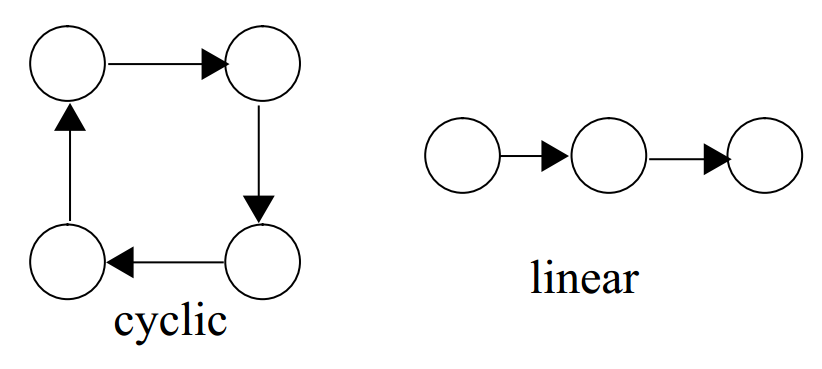
\includegraphics[height=100px]{artigos/1994_Synthesizing_Parameterized_Motions_egw94/fig2.png}
  \caption{Duas possíveis topologias para o grafo de pose.}
  \label{fig:1994:synthesizing:fig2}
\end{figure}

Grafos de pose são grafos orientados que representam as transições entre as diferentes configurações desejadas do modelo articulado.

Os parametros dos controladores podem ser definidos manualmente ou sintetizados. No artigo, o autor cita o uso da técnica de otimização em duas fases para gerar os parâmetros. Então é gerado um grafo de controle da pose, onde cada estado representa uma posição no qual o controlador deverá tentar atingir. As posições são representadas por um conjunto de graus de liberdade dos atuadores, que contém informação dos valores máximos e mínimos para cada um, como visto na figura \ref{fig:1994:synthesizing:fig12}.

\begin{figure}[ht]
  \centering
  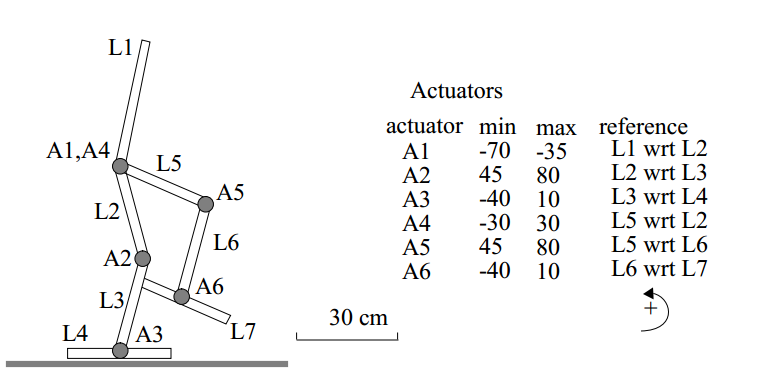
\includegraphics[height=150px]{artigos/1994_Synthesizing_Parameterized_Motions_egw94/fig12.png}
  \caption{Modelo simples com duas pernas representando o "estado zero" e todos os graus de liberdade para atingir a pose vista.}
  \label{fig:1994:synthesizing:fig12}
\end{figure}

Os experimentos foram realizados utilizando um modelo 2D, porém o autor demonstra otimismo para expandir a técnica para um modelo 3D. Para atingir maior realismo da simulação, o modelo deve ser mais discretizado e contar com mais tipos de atuadores para ter uma melhor representação da musculatura do individuo.

Para criar uma animação, um animador precisa primeiramente criar uma figura articulada, especificar a topologia do grafo de controle de pose e decidir qual métrica será usada para avaliar o desempenho da animação. Essa métrica normalmente é uma combinação de valores como velocidade, distância percorrida e energia consumida no processo.

Para movimentos periódicos, um grafo cíclico é necessário. Dado um período desejado T e um numero n de transições, o tempo de transição é calculado fazendo $ \frac{T}{n} $. Para movimentos aperiódicos, um grafo linear é definido a priori.

Essas informações são utilizadas para reduzir drasticamente o espaço de busca, e consequentemente o tempo, do processo de síntese. O processo de síntese produz uma pose para cada estado do gráfico que gere uma animação desejada.

A técnica de busca utilizada, em duas fases, consiste em gerar controladores, testá-los, e a partir dos resultados, modificá-los e testá-los novamente até que um resultado desejado seja atingido. Os controladores gerados são avaliados através da métrica definida inicialmente. 

\begin{figure}[ht]
  \centering
  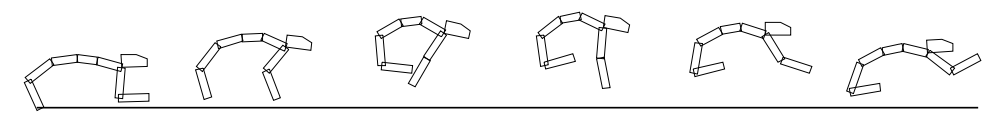
\includegraphics[width=300px]{artigos/1994_Synthesizing_Parameterized_Motions_egw94/fig3.png}
  \caption{Modelo de cheetah exemplificando o resultado de um movimento cíclico.}
  \label{fig:1994:synthesizing:fig3}
\end{figure}

Para um caso de teste, foram gerados na primeira fase 100 controladores, dos quais apenas 10 foram selecionados para prosseguir. Para a segunda fase, parâmetros dos controladores foram perturbados utilizando um delta fixo de 5\% o valor da amplitude do grau de liberdade, aleatoriamente. Então é decidido se a mudança será mantida ou não, baseado novamente na métrica. Para conseguir tais resultados, arrefecimento simulado ou método do gradiente podem ser utilizados.
O resultado pode ser observado na figura \ref{fig:1994:synthesizing:fig3}.

\begin{figure}[ht]
  \centering
  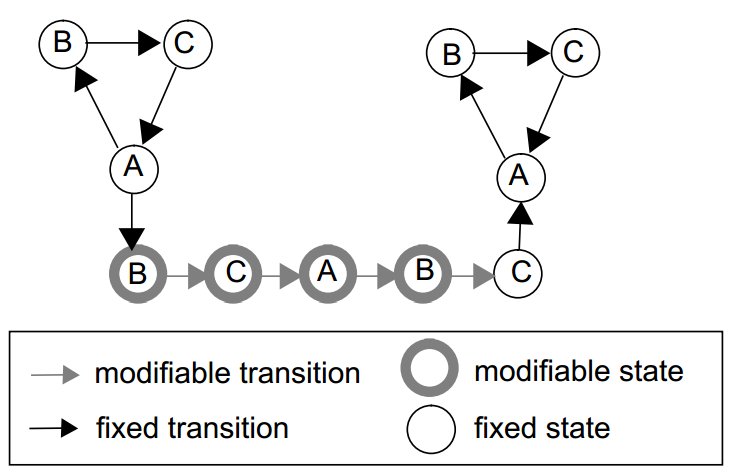
\includegraphics[height=100px]{artigos/1994_Synthesizing_Parameterized_Motions_egw94/fig4.png}
  \caption{Grafo de controle de pose representando o salto do Luxo, mascote da Pixar.}
  \label{fig:1994:synthesizing:fig4}
\end{figure}

Muitos movimentos aperiodicos interessantes podem ser derivados a partir de movimentos periódicos. Na figura \ref{fig:1994:synthesizing:fig4}, vemos que existe uma porção cíclica, representando um movimento periódico. Dado uma condição, é possível sair do ciclo através da transição do meio, e retornar em seguida. Dessa forma, Luxo faz um movimento de saltos, e pode interromper o ciclo para fazer um pulo longo, e retornar ao seu movimento anterior.

%parametrização de movimento

Parametrização de movimento é uma forma de abstrair todos os possíveis tipos de movimentação. É um passo necessário para construção de mecânicas de controle mais complexas abstraindo determinadas noções de movimento. O animador já tem o poder de influenciar o resultado da animação modificando o modelo utilizado e a métrica da otimização. 

A relação entre os parâmetros do grafo de controle de posição e a animação resultante é bastante complexa. Dada a dificuldade de descrever essa relação de forma analítica, podemos observar o impacto que determinadas mudanças têm no resultado final da simulação. O que observamos é que pequenas mudanças nos parâmetros causam pequenas mudanças no movimento final. Como resultado dessa propriedade, podemos interpolar duas posições desejadas interpolando seus parâmetros de controle.

\begin{figure}[ht]
  \centering
  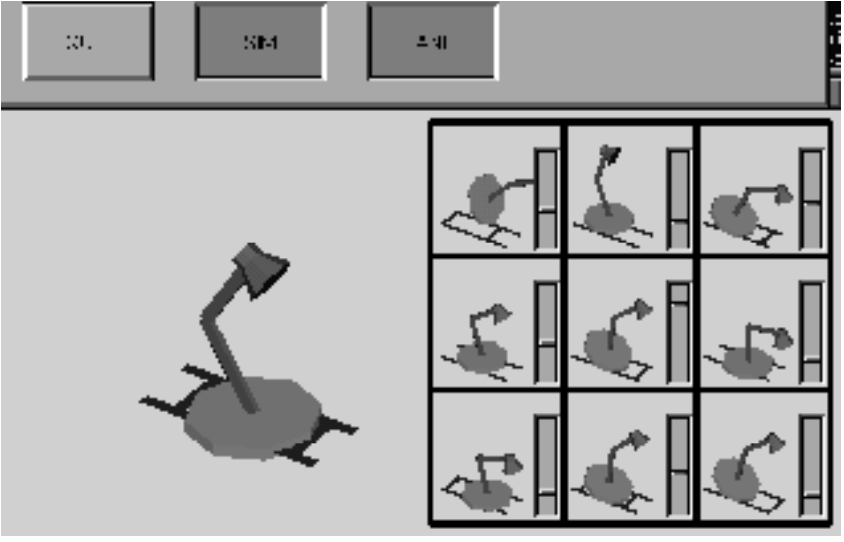
\includegraphics[height=150px]{artigos/1994_Synthesizing_Parameterized_Motions_egw94/fig10.png}
  \caption{É possivel ver no espaço da esquerda o movimento original de Luxo. Na direita, uma paleta de sugestões de possíveis modificações que podem ser feitas na animação.}
  \label{fig:1994:synthesizing:fig10}
\end{figure}

Uma forma de gerar variações do movimento é sortear um parâmetro por vez, e modificá-lo até que um critério de semelhança entre as posições não seja mais atendida.
O artigo cita o uso da velocidade como critério de semelhança, onde uma diferença de até +-30\% é classificada como semelhante.

Assim que as variações de movimento são geradas, o resultado pode ser utilizado como uma "paleta" de poses, como ilustrado na figura \ref{fig:1994:synthesizing:fig10} para o animador, interativamente, definir o comportamento desejado da animação. 

É importante notar que o resultado da interpolação dos parâmetros é diferente do caso em que se interpola valores cinemáticos. No caso da interpolação dos parâmetros, as leis da física serão mantidas no resultado final.

%\begin{figure}[ht]
%  \centering
%  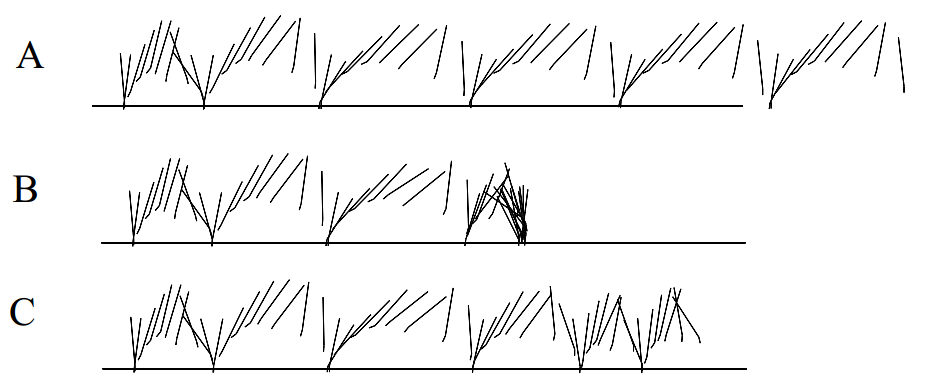
\includegraphics[height=100px]{artigos/1994_Synthesizing_Parameterized_Motions_egw94/fig6.png}
%  \caption{xxx}
%  \label{fig:1994:synthesizing:fig6}
%\end{figure}
%
%\begin{figure}[ht]
%  \centering
%  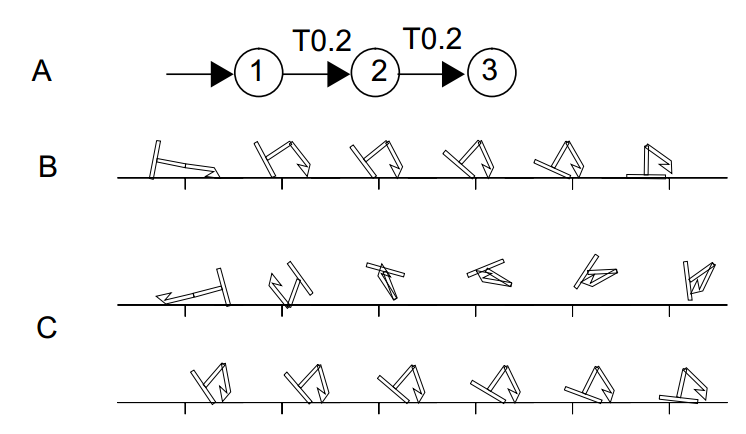
\includegraphics[height=100px]{artigos/1994_Synthesizing_Parameterized_Motions_egw94/fig7.png}
%  \caption{xxx}
%  \label{fig:1994:synthesizing:fig7}
%\end{figure}
%
%\begin{figure}[ht]
%  \centering
%  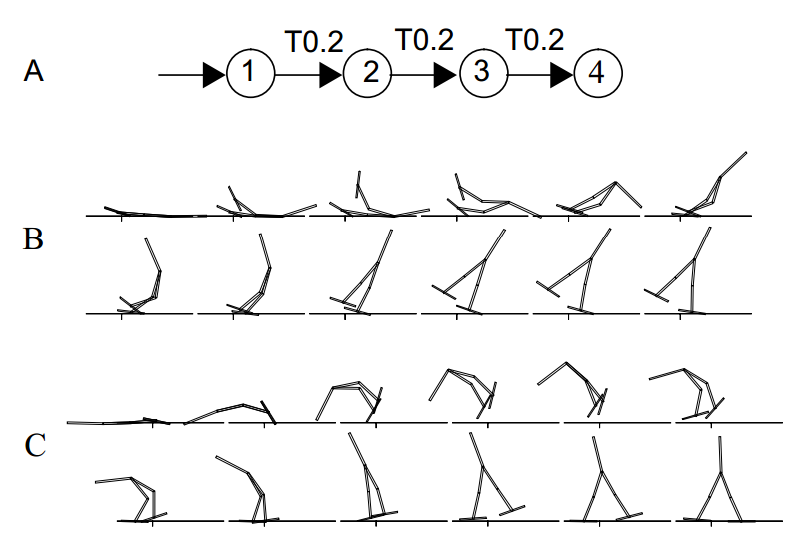
\includegraphics[height=100px]{artigos/1994_Synthesizing_Parameterized_Motions_egw94/fig8.png}
%  \caption{xxx}
%  \label{fig:1994:synthesizing:fig8}
%\end{figure}
%
%\begin{figure}[ht]
%  \centering
%  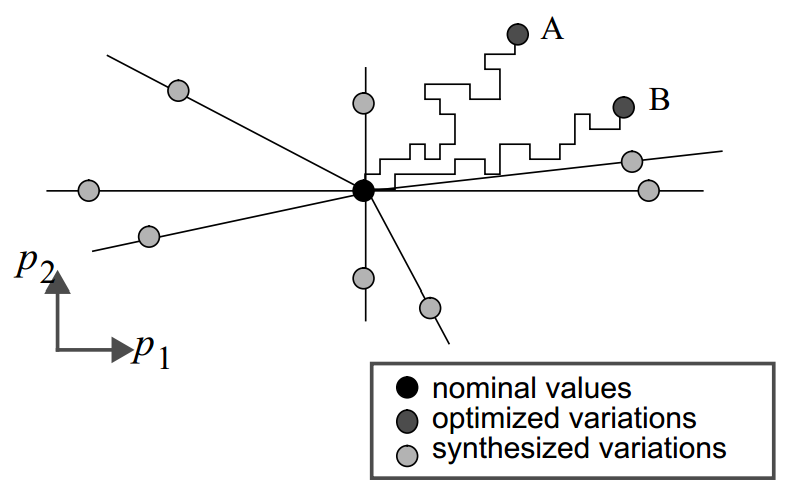
\includegraphics[height=100px]{artigos/1994_Synthesizing_Parameterized_Motions_egw94/fig9.png}
%  \caption{xxx}
%  \label{fig:1994:synthesizing:fig9}
%\end{figure}
%
%\begin{figure}[ht]
%  \centering
%  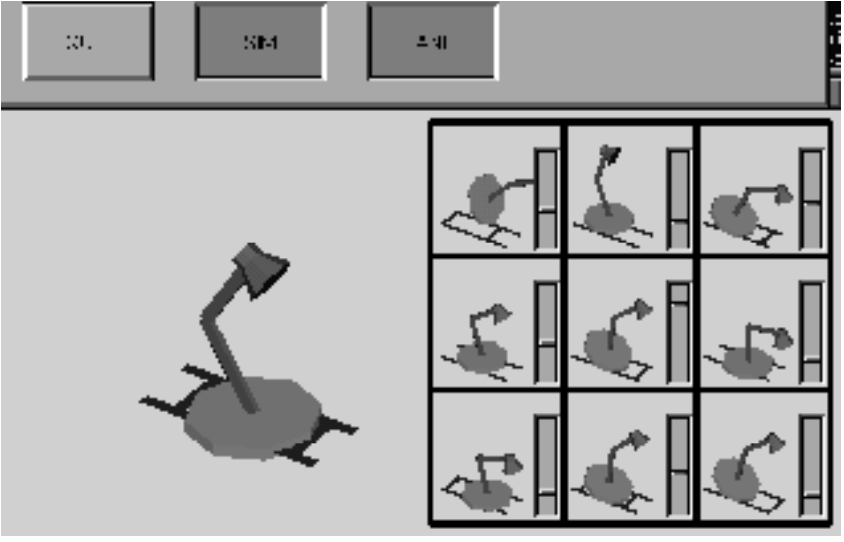
\includegraphics[height=100px]{artigos/1994_Synthesizing_Parameterized_Motions_egw94/fig10.png}
%  \caption{xxx}
%  \label{fig:1994:synthesizing:fig10}
%\end{figure}
%
%\begin{figure}[ht]
%  \centering
%  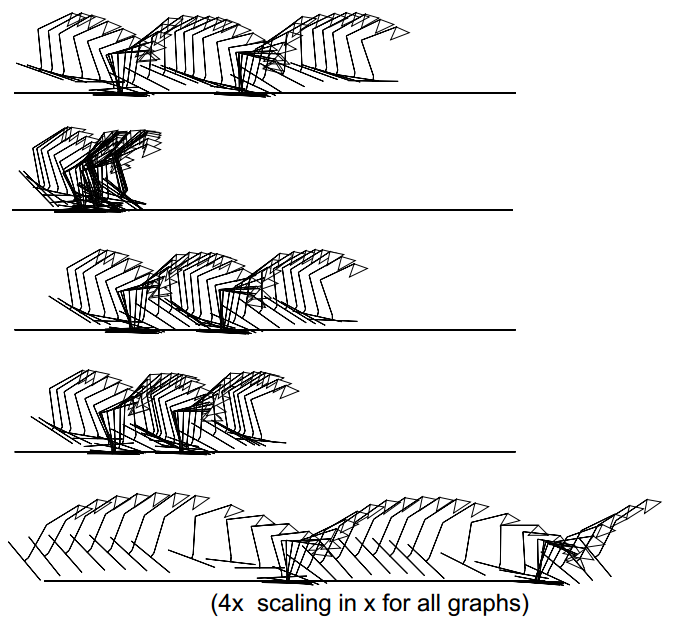
\includegraphics[height=100px]{artigos/1994_Synthesizing_Parameterized_Motions_egw94/fig11.png}
%  \caption{xxx}
%  \label{fig:1994:synthesizing:fig11}
%\end{figure}

% ..........................................................
\subsubsection{Resultados}
O uso de grafo de controle de pose demonstrou ser uma representação flexivel para criação de movimentos periódicos e aperiódicos. Quando usado com transições de estado baseados em tempo, pode gerar movimentos complexos que são graciosos e realistas.
Uma nova forma de utilizar otimização para sintese de movimento foi apresentada, melhorando aspectos como a criação de movimentos fisicamente realistas mais complexos, ciclicos ou aciclicos, de forma eficiente. Isso facilita o processo de projetar o controlador em alto nivel e os movimentos baseados em física.

% ============================================================================
\subsection{Pontos fortes} %no máximo três
\begin{itemize}
  \item Nova forma de utilizar otimização para síntese de movimentos.
  \item Grafo de controle de pose mais complexos, para movimentos cíclicos e aciclicos.
  \item Parametrização da solução que tornou possível um controle de mais alto nível sobre a simulação.
\end{itemize}  

% ============================================================================
\subsection{Limitações} %no máximo três
\begin{itemize}
  \item Movimentos que não são dinamicamente estáveis sem o uso de feedback não podem ser controlados em um ciclo fechado. Tais movimentos complexos necessitam de feedback contínuo do estado.
  \item A sintese do grafo de controle da pose continua um processo caro computacionalmente.
  \item 
\end{itemize} 


% ============================================================================
\subsection{Avaliação}
%\textbf{(a) Avanço considerável (\textit{Breakthrough}).}
 \textbf{(b) Contribuição significativa.}
% \textbf{(c) Contribuição modesta.}
% \textbf{(d) Contribuição fraca.}
% \textbf{(e) Sem contribuição.}
É possivel agora gerar movimentos fisicamente realistas com um algoritmo relativamente genérico. Dadas as restrições da técnica, é possível com algumas parametrizações gerar um grafo de controle de pose que resulte na animação desejada, sem a necessidade de manipular o grafo explicitamente.

Alguns artigos anteriores já haviam tentado algo parecido, porém com mais limitações na técnica e com desempenho inferior.

% ============================================================================
\subsection{Problema em aberto}
 \begin{itemize}
   \item Adicionar equilibrio resolveria o problema dos movimentos complexos?
   \item Otimizar o processo de sintese do grafo de controle de pose.
   \item Como conseguir movimentos mais autonomos e complexos com a sintese
   \item Extender a técnica para movimentos e modelos mais complexos e utilizando 3 dimensões ao invés de 2.
   \item Explorar a melhor forma de integrar informação sensorial aos grafos de controle de pose.
 \end{itemize}  

% ============================================================================
\subsection{Aspecto obscuro}
 \begin{itemize}
   \item É preciso ver como a técnica se comporta em animações de objetos mais complexos, ou seja, objetos com mais graus de liberdade.
 \end{itemize}  

\chapter{Mês de setembro}
%\section{\textit{Virtual Wind-up Toys for Animation}}

% ============================================================================
\subsection{Referência completa do artigo}

\begin{itemize}
  \item \textbf{Autores:} Mitchel van de Panne, Ryan Kim, Eugene Fiume
  \item \textbf{Local:} Department of Computer Science and Electrical Engineering, University of Toronto, Canada
  \item \textbf{\textit{Journal}:} xxx [Qualis XXX]
  \item \textbf{Data:} xxx
  \item \textbf{Referência:} \citeonline{bib:1994:winduptoys}
\end{itemize}


% ============================================================================
\subsection{Resumo}
% ..........................................................
\subsubsection{Abstract}
We propose a new method of automatically finding periodic modes of locomotion for arbitrary articulated figures. Cyclic pose control graphics are used as our control representation. These specifically constrain the controller synthesis process to only those controllers producing periodic driving functions. It is shown that stochastic generate-and-test techniques work well with this representation. Several choices that arise in this synthesis technique are explored. The impact of the design of the physical models upon the motions produced is examined. Lastly, the motions produced are analysed by looking at their bifurcation diagrams.
% ..........................................................
\subsubsection{Motivação}
Este artigo apresenta uma tecnica de controladores que permite criação de movimentos complexos e que respeitam as restrições físicas impostas, tentando manter a solução livre de casos específicos.
% ..........................................................
\subsubsection{Propósito do artigo}

Nele é apresentada uma forma de encontrar modos periódicos de locomoção para produzir animações fisicamente realistas para um modelo qualquer.

% ..........................................................
\subsubsection{Técnicas utilizadas} 
 \begin{itemize}
   \item Controladores
   \item Grafo de controle de pose
 \end{itemize}  
xxx

% ..........................................................
\subsubsection{Contribuição em relação a artigos anteriores} %mais ou menos 10 linhas
% \begin{itemize}
%   \item xxx
% \end{itemize}  
xxx

% ============================================================================
\subsection{Metodologia}
% Descreva um pouco mais detalhadamente a metodologia e os resultados do artigo. 
% Inclua as figuras que achar mais relevantes.



% ..........................................................
\subsubsection{Resultados}
asd

% ============================================================================
\subsection{Pontos fortes} %no máximo três
\begin{itemize}
  \item xxx
  \item xxx
  \item xxx
\end{itemize}  

% ============================================================================
\subsection{Limitações} %no máximo três
\begin{itemize}
  \item xxx
  \item xxx
  \item xxx
\end{itemize} 


% ============================================================================
\subsection{Avaliação}
\textbf{(a) Avanço considerável (\textit{Breakthrough}).}
% \textbf{(b) Contribuição significativa.}
% \textbf{(c) Contribuição modesta.}
% \textbf{(d) Contribuição fraca.}
% \textbf{(e) Sem contribuição.}
Justificativa.

% ============================================================================
\subsection{Problema em aberto}
% \begin{itemize}
%   \item xxx
% \end{itemize}  
xxx

% ============================================================================
\subsection{Aspecto obscuro}
% \begin{itemize}
%   \item xxx
% \end{itemize}  
xxx

\section{\textit{Tracking and Modifying Upper-body Human Motion Data with Dynamic Simulation}}

% ============================================================================
\subsection{Referência completa do artigo}

\begin{itemize}
  \item \textbf{Autores:} Victor B. Zordan, Jessica K. Hodgins
  \item \textbf{Local:} College of Computing and Graphics, Visualization and Usability Center, Georgia Institute of Technology
  \item \textbf{\textit{Journal}:} EUROGRAPHICS [Qualis A2]
  \item \textbf{Data:} Sept 1999
  \item \textbf{Referência:} \citeonline{bib:1999:upperbody}
\end{itemize}


% ============================================================================
\subsection{Resumo}

\subsubsection{Abstract}
Character animations produced with motion capture data have many of the stylistic details seen in human motion while those generated with simulation are physically realistic for the dynamic parameters of the character. We combine these two approaches by tracking and modifying human motion capture data using dynamic simulation and constraints. The tracking system generates motion that is appropriate for the graphical character while maintaining characteristics of the original human motion. The system imposes contact and task constraints to add dynamic impacts for interactions with the environment and to modify motions at the behavior level. The system is able to edit motion data to account for changes in the character and the environment as well as create smooth transitions between motion capture sequences. We demonstrate the power of combining these two approaches by tracking data for a variety of upper-body motions and by animating models with differing kinematic and dynamic parameters.

% ..........................................................
\subsubsection{Motivação}
A tecnica descrita no artigo indica uma maneira de combinar as tecnicas de captura de movimento e simulação dinamica para composição de animações que aparentam ser naturais e ao mesmo tempo respeitem as restrições físicas. Isso permite adaptar movimentos de captura para novas situações e fazer uma simulação reativa ao meio em que ela acontece e aos eventos que ocorrem.
% ..........................................................
\subsubsection{Propósito do artigo}
Simulação dinâmica garante uma animação fisicamente correta e se adapta naturalmente às mudanças de restrições do meio. Porém não é fácil simular os detalhes minunciosos da movimentação natural humana com um modelo simplificado do esqueleto e da musculatura.
A técnica de captura de movimento fornece um banco de dados com animações realistas e representam bem a naturalidade do movimento humano, ou de qualquer "ator" que tenha seu movimento capturado. Movimentos desse tipo são difíceis de se gerar proceduralmente, e por isso a técnica de captura ainda é a melhor para esse tipo de resultado.
% ..........................................................
\subsubsection{Técnicas utilizadas} 
\begin{itemize}
  \item Motion Capture
  \item Simulação Dinâmica
  \item Cinemática Inversa
  \item Cinemática Direta
  \item Controlador de trajetória
  \item Controlador de equilíbrio
\end{itemize}  

% ..........................................................
\subsubsection{Contribuição em relação a artigos anteriores} %mais ou menos 10 linhas
 \begin{itemize}
   \item Artigos anteriores tentaram combinar as técnicas mas utilizando abordagens diferentes. Neste artigo um modelo detalhado e completamente simulado foi utilizado no lugar de uma versão simplificada. Isso permite maior realismo na animação final.
   \item
 \end{itemize}  

% ============================================================================
\subsection{Metodologia}
% Descreva um pouco mais detalhadamente a metodologia e os resultados do artigo. 
% Inclua as figuras que achar mais relevantes.

\begin{figure}[ht]
  \centering
  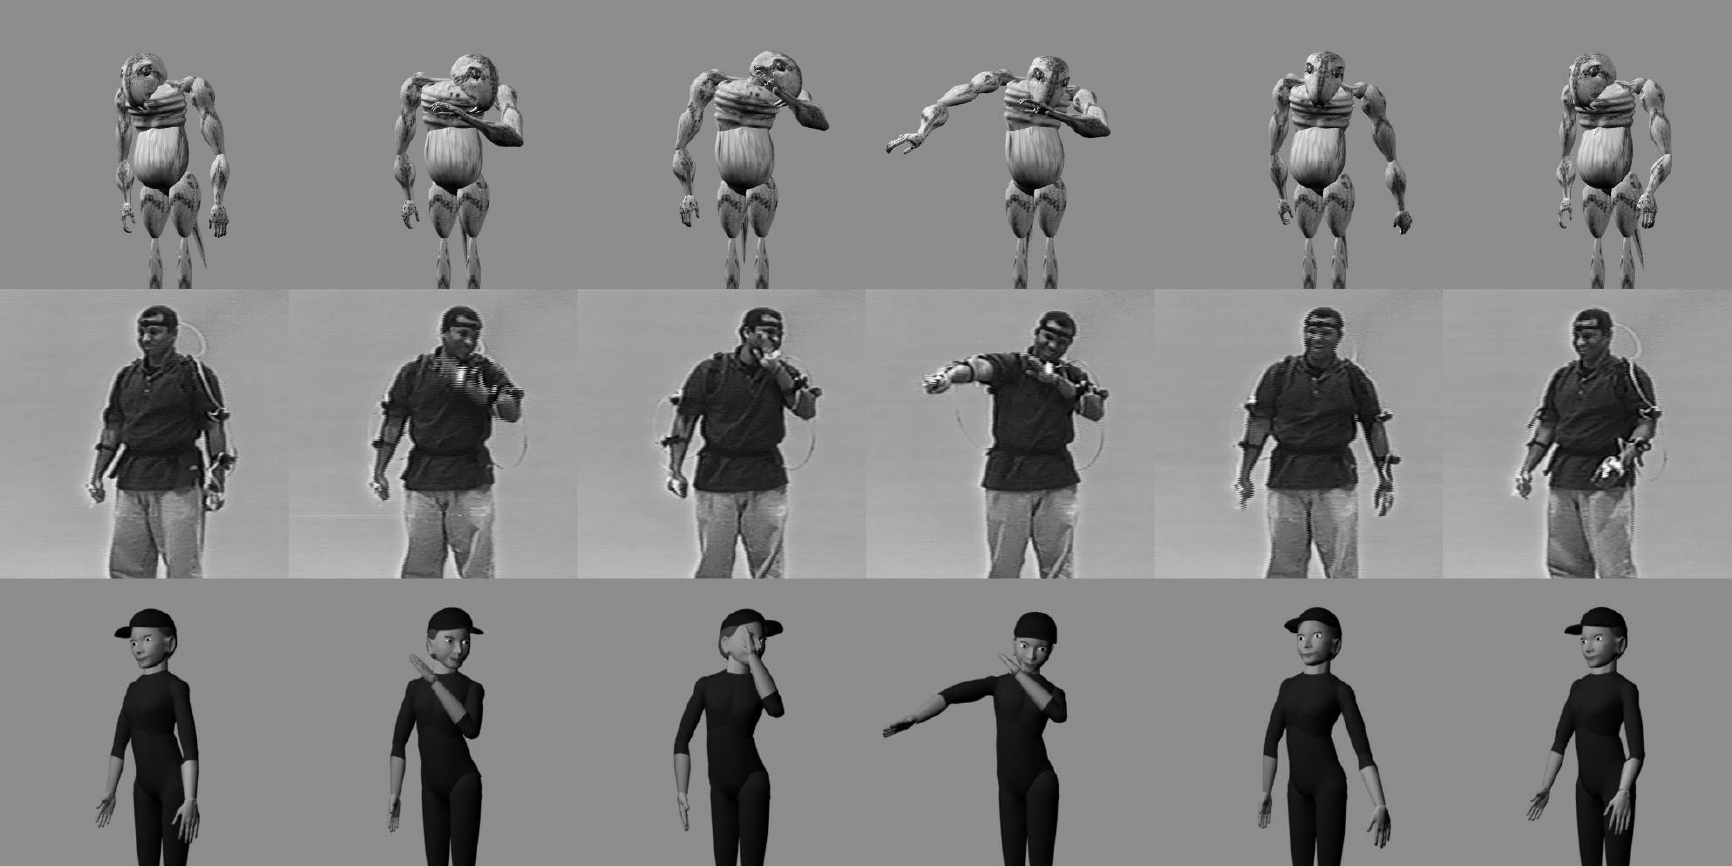
\includegraphics[height=150px]{artigos/1999_Tracking_and_Modifying_Upper-body_Human_Motion_Data_with_Dynamic_Simulation_zordan_TMU/fig_mocap.png}
  \caption{Captura de movimento mapeada em personagens virtuais.}
  \label{fig:1999:upperbody:fig1}
\end{figure}


\subsubsection{Motion Capture}

Existem diversas técnicas de motion capture, que tentam mapear movimentos reais para modelos virtuais. No artigo, eles utilizaram um ator com sensores de movimento no corpo. O resultado do mapeamento pode ser visto na figura \ref{fig:1999:upperbody:fig1}, onde no meio acompanhamos o processo de captura, e ao redor podemos ver o mesmo movimento mapeado em personagens com características físicas diferentes.

\begin{figure}[ht]
  \centering
  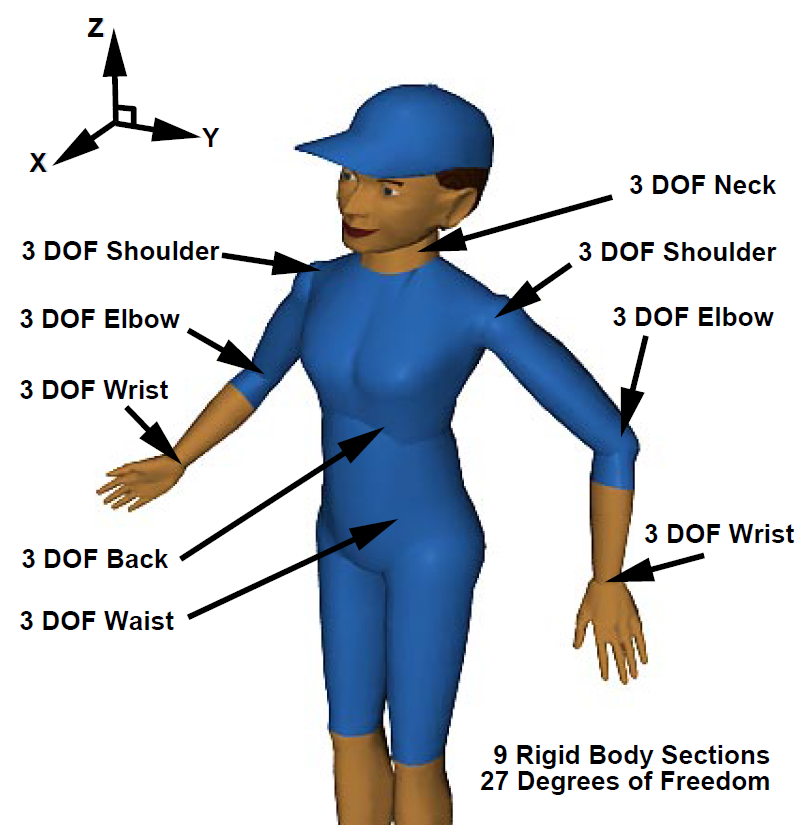
\includegraphics[height=150px]{artigos/1999_Tracking_and_Modifying_Upper-body_Human_Motion_Data_with_Dynamic_Simulation_zordan_TMU/fig_model.png}
  \caption{Este modelo tem 27 graus de liberdade controlados, com pernas estáticas. Outro modelo tem apenas 24 graus de liberdade, excluindo a articulação das costas. O modelo de corpo inteiro possui 48 graus de liberdade, com juntas adicionais nas pernas para manter o equilíbrio.}
  \label{fig:1999:upperbody:fig2}
\end{figure}

\subsubsection{Combinação das técnicas}

Para conseguir o resultado de combinar as duas ténicas, três adições são feitas ao sistema. Primeiramente, um gerenciador de colisões, para detectar interações com o ambiente. Segundo, controladores são adicionados. Esses controladores podem corrigir a movimentação do personagem diante das interações físicas, modificar a movimentação do personagem a nivel comportamental, adicionar noção de equilíbrio para manter o personagem de pé e animar graus de liberdade que não foram capturados previamente. Terceiro, os inputs de captura podem ser modificados e combinados para gerar novos movimentos, que juntamente com a simulação de física, se provaram suaves e realistas.

\begin{figure}[ht]
  \centering
  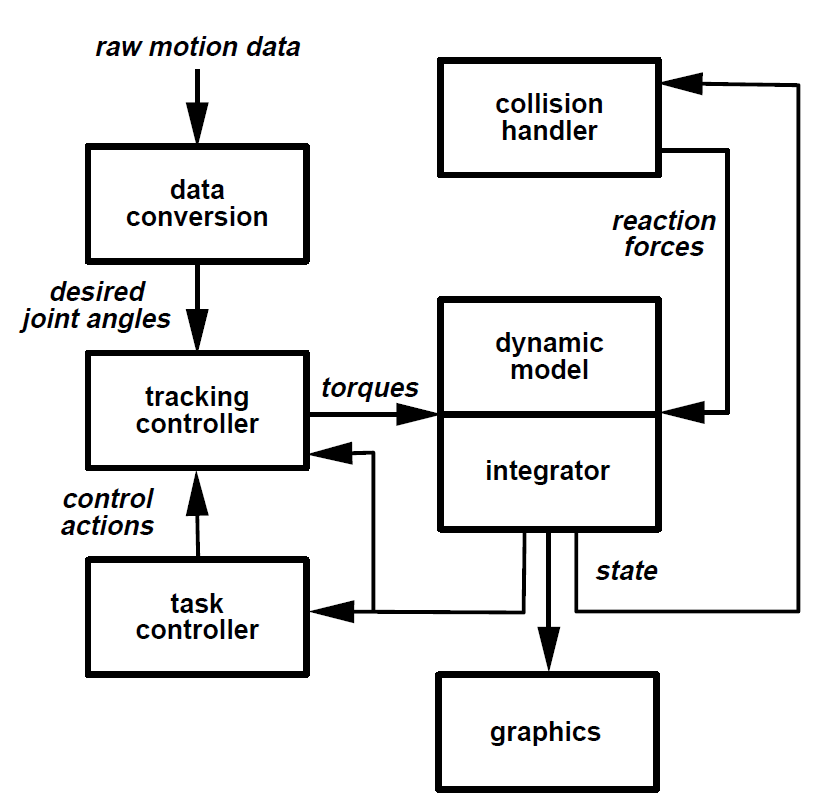
\includegraphics[height=150px]{artigos/1999_Tracking_and_Modifying_Upper-body_Human_Motion_Data_with_Dynamic_Simulation_zordan_TMU/fig_layout.png}
  \caption{O dado bruto de captura é convertido em angulos para as juntas, e são utilizados como valor a ser atingido pelos controladores de trajetória. Um controlador de tarefa e um gerenciador de colisão podem ser adicionados para gerar movimentos mais complexos e direcionar o comportamento.}
  \label{fig:1999:upperbody:fig3}
\end{figure}

\subsubsection{Simulação dinâmica e controle de trajetória}

Para que o modelo siga a animação capturada, um controlador de trajetória é utilizado. Ele aplica forças nas juntas de modo que o modelo tente acompanhar o movimento capturado. Porém, junto a este controlador, a simulação de física está presente para trazer as restrições do mundo para a simulação. Este caso é apropriado para gestos simples ou quando há uma correspondência boa entre o ator capturado e o personagem gráfico. O esquema pode ser visto na \ref{fig:1999:upperbody:fig3}.
A técnica citada é utilizada na parte superior do corpo. Para a parte inferior, o personagem pode ser mantido estático ou utilizar um controlador de equilíbrio para aumentar o realismo e manter o personagem de pé. A figura \ref{fig:1999:upperbody:fig2} mostra um exemplo de modelo que pode ser utilizado para a simulação, indicando os graus de liberdade de cada junta.
Para os cálculos, o modelo precisa ter valores de massa e momento de inércia. Para este trabalho, os valores foram estimados a partir dos modelos tridimensionais e valores supostos de densidade.
Por conta do custo elevado do cálculo de colisão, foram consideradas apenas colisões em partes do corpo que eram de se esperar que colidissem durante a simulação. Colisões entre partes do mesmo corpo foram desconsideradas.
O angulo e a posição de cada marcador é fornecida pelo sistema de captura, e assim é possivel calcular os angulos desejados em cada junta. O angulo é calculado pela fórmula:
\begin{equation}
  \label{eq:1999:upperbody:calc_angulo}
  \Theta_{desired} = \Theta_{ii}^T\Theta_{io}
\end{equation}
Onde $ \Theta_{ii} $ representa a matriz de transformação do objeto que aparece anteriormente na arvore hierárquica (objeto pai), e $ \Theta_{io} $ o objeto que aparece posteriormente (objeto filho). A raiz da árvore foi considerada na pélvis.
Para o cálculo do torque a ser aplicado em cada junta, a seguinte formula se aplica:
\begin{equation}
  \label{eq:1999:upperbody:calc_torque}
  \tau = k ( \theta_{desired} - \theta_{actual} ) - k_d ( \dot{\theta}_{actual} )
\end{equation}
onde $\theta_{actual}$ e $\theta_{desired}$ correspondem aos angulos atual e desejado da junta, e $\dot{\theta}_{actual}$ é a velocidade atual da junta. $k$ e $k_d$ são termos de ganho e amortecimento. O sistema funcionará como uma mola e um amortecedor, definindo um "músculo de primeira ordem".
Não são estabelecidos limites para as juntas pois considera-se que o movimento de captura respeita as restrições naturais do movimento.
O controlador então é ajustado para minimizar o erro $\epsilon$:
\begin{equation}
  \label{eq:1999:upperbody:calc_stiffness}
  \epsilon = \sum{||\theta_{desired}-\theta_{actual}||}
\end{equation}
Dessa forma o controlador irá gerar um movimento mais aproximado da captura de input.

\subsubsection{Restrições}

Restrições foram classificadas como restrições de ambiente, restrições de tarefas. Um exemplo de restrição dinâmica de ambiente poderia ser um personagem batendo em um tambor. O tambor faz parte da cena, e ao atingir, uma força impedirá a mão de atravessar o tambor, fazendo um movimento reativo realista. Uma restrição de tarefa seria por exemplo um personagem segurando um cajado, e tentando equilibrar o mesmo enquanto sacode no ar. Para isso, é colocado um controlador de tarefa na mão do personagem para dar um ar de realismo no movimento, como se ele realmente estivesse segurando o peso do cajado. Outro exemplo é o controlador usado nas pernas que tentam manter o personagem ereto enquanto executa as movimentações na parte superior do corpo, mantendo o centro de massa dentro da região dos pés.

\subsubsection{Modificando Inputs}
A ideia é modificar os dados de captura para gerar novos movimentos que não estavam inicialmente previstos, adaptando a novas situações. Uma possibilidade é o uso de cinemática inversa, como no caso das crianças batendo palmas. O movimento foi capturado a partir de um adulto, mas devido as diferentes proporções dos corpos, um novo offset para as mãos teve de ser definido. A solução retratada no artigo mantém a mão com a mesma orientação, mudando sua posição para a desejada, e então o sistema é resolvido. É possível utilizar cinematica inversa também para modificar a velocidade de um movimento, mantendo o realismo. Existe um limite em que o sistema pode parar de funcionar e detectar contatos. Nesse caso, aumentar a duração do offset pode ajudar a contornar um pouco este problema.
Além disso, é possível combinar diferentes animações capturadas, concatenando ou interpolando, e então usar a sequencia final na simulação. Este é um problema comum a respeito de captura de movimentos e existem diversas soluções para isso. Para o exemplo das palmas, foi utilizada uma posição chave, e fazer que cada movimento comece e termine nessa posição. Isso permite uma solução imediata da concatenação de movimentos pois uma transição é imediata. Uma solução mais geral permite que qualquer animação se encaixe em outra, independentemente da sua configuração inicial e final. Para isso é dada uma função de peso que varia com o tempo, permitindo que uma animação transicione para a outra suavemente. Isto é feito com a seguinte fórmula:
\begin{equation}
  \label{eq:1999:upperbody:calc_stiffness}
  \theta_r(t) = \theta_a(t)(1-\omega(t)) +   \theta_b(t)\omega(t), 0<=\omega(t)<=1, t_0 <= t <= t_1
\end{equation}
Isso é uma $slerp$ entre cada angulo $\theta_a$ e $\theta_b$ em um determinado tempo $t$. A função $\omega$ utilizada pode ser uma função senoide de $ease in/ease out$.
O movimento resultante, por ser uma combinação de dois movimentos reais, acaba se tornando um movimento realistico.
% ..........................................................
\subsubsection{Resultados}
Um sistema que utiliza o modelo dinamico para seguir e modificar dados de captura de movimento para a parte superior do corpo foi apresentada, junto com diversos exemplos que demonstram o poder da técnica. É dificil ter naturalidade e estilo como métricas, e isso torna uma avaliação crítica do trabalho algo complicado. Uma possivel métrica é a comparação entre movimentos gerados e movimentos capturados brutos de mesma natureza que tenham sido capturados. Foi observado que o movimento pode apresentar uma suavidade maior que o movimento capturado. Isso faz com que algumas tarefas se tornem impossíveis de alcançar. Para resolver o problema, foi utilizada cinemática inversa. 
Varias sugestões foram propostas em situações onde o sistema não funciona muito bem. E apesar da solução apresentada não resolver o problema geral da simulação com dados de captura de movimento, é um passo considerável em relação a tentativas anteriores de produzir esse tipo de animação.

% ============================================================================
\subsection{Pontos fortes} %no máximo três
\begin{itemize}
  \item Combina o melhor da captura de movimento e da simulação física
  \item Personagem completamente simulado, permite animações mais realistas que artigos anteriores.
  \item Simulação detalhada da parte superior do corpo, que é relevante por conta da expressividade dos braços e da cabeça humana.
\end{itemize}  

% ============================================================================
\subsection{Limitações} %no máximo três
\begin{itemize}
  \item Outros artigos permitem simulações mais complexas, como saltos e corridas, porém eles utilizam um modelo simplificado de simulação.
  \item É restrito à parte superior do corpo, sendo a simulação da parte de baixo apenas para manter o equilíbrio, ou uma animação fixa.
  \item Para alguns movimentos é necessário o uso de cinemática inversa para posicionar elementos do corpo em posições desejadas, tornando o processo automático de sintese da animação menos automático.
\end{itemize} 

% ============================================================================
\subsection{Avaliação}
%\textbf{(a) Avanço considerável (\textit{Breakthrough}).}
 \textbf{(b) Contribuição significativa.}
% \textbf{(c) Contribuição modesta.}
% \textbf{(d) Contribuição fraca.}
% \textbf{(e) Sem contribuição.}

O artigo diminui consideravelmente a quantidade de input necessário para gerar uma animação fisicamente realista a partir de dados de captura, além de permitir modelos mais complexos e animações mais expressivas da parte superior do corpo humano, que representa melhor essa expressividade do corpo.

% ============================================================================
\subsection{Problema em aberto}
 \begin{itemize}
   \item Expandir a solução para animações mais complexas e utilizando o corpo inteiro com o mesmo nível de complexidade.
   \item Extrair informação relevante sobre o movimento a partir do dado de captura para criar novos comportamentos.
 \end{itemize}  

% ============================================================================
\subsection{Aspecto obscuro}
 \begin{itemize}
   \item Não fica claro quando a cinemática inversa deve ser utilizada para gerar um movimento desejado. Ela parece ser essencial para alguns tipos de atividades desejadas.
   \item A métrica para avaliar a técnica utilizada pelo autor. Mesmo tendo dado algumas sugestões, parece algo bem subjetivo.
 \end{itemize}  

\section{\textit{Motion capture-driven simulations that hit and react}}

% ============================================================================
\subsection{Referência completa do artigo}

\begin{itemize}
  \item \textbf{Autores:} Victor B. Zordan, Jessica K. Hodgins
  \item \textbf{Local:} College of Computing and GVU Center, Georgia Institute of Technology
  \item \textbf{\textit{Journal}:} SIGGRAPH Symposium on Computer Animation [Qualis A2]
  \item \textbf{Data:} 21-26 July 2002
  \item \textbf{Referência:} \citeonline{bib:2002:cms}
\end{itemize}

% ============================================================================
\subsection{Resumo}

\subsubsection{Abstract}

Controllable, reactive human motion is essential in many video games and training environments. Characters in these applications often perform tasks based on modified motion data, but response to unpredicted events is also important in order to maintain realism. We approach the problem of motion synthesis for interactive, human-like characters by combining dynamic simulation and human motion capture data. Our control systems use trajectory tracking to follow motion capture data and a balance controller to keep the character upright while modifying sequences from a small motion library to accomplish specified tasks, such as throwing punches or swinging a racket. the system reacts to forces computed from a physical collision model by changing stiffness and damping terms. The free-standing, simulated humans respond automatically to impacts and smoothly return to tracking. We compare the resulting motion with video and recorded human data.

% ..........................................................
\subsubsection{Motivação}
Para conseguir movimentos realistas, é interessante estudar a técnica de captura de movimentos e como os dados de captura podem ser modificados para adequar a animação a cada situação, como reação a um obstáculo móvel.

% ..........................................................
\subsubsection{Propósito do artigo}

A ideia do artigo é partir de um banco de movimentos previamente capturados, que possuem características naturais e trazem menos estranhamento ao serem vistos, e tentar obter uma animação final, fisicamente realista, com transições suaves entre as poses de forma que seja gerada uma animação desejada.

% ..........................................................
\subsubsection{Técnicas utilizadas} 
\begin{itemize}
  \item Motion Capture
  \item Controladores
  \item Cinemática Inversa
  \item Blending de animações
\end{itemize}  

% ..........................................................
\subsubsection{Contribuição em relação a artigos anteriores} %mais ou menos 10 linhas
 \begin{itemize}
   \item x
 \end{itemize}  

% ============================================================================
\subsection{Metodologia}
% Descreva um pouco mais detalhadamente a metodologia e os resultados do artigo. 
% Inclua as figuras que achar mais relevantes.

\subsubsection{Introdução}

O objetivo é combinar dois objetivos, muitas vezes conflitantes: permanecer proximo o suficiente do dado capturado original, para manter características importantes da animação real e desviar o suficiente deste resultado para atingir outro objetivo, dada uma tarefa.

\subsubsection{Editando motion capture}

Diversas tecnicas existem para essa tarefa. Interpolação de keyframes, adaptando o movimento para um novo personagem mantendo os contatos e alterando a dinâmica da animação, usando b-splines. Para a implementação sugerida pelo artigo, eles realizam pequenas edições na animação original, e essa animação modificada será o input para a simulação que é feita em seguida.
Outro problema existente é como combinar mais de uma animação. Uma possibilidade seria decompor dois movimentos bem diferentes em bandas de frequencia e permitir o usuário controlar o blending entre essas frequencias. Outra possibilidade é utilizar uma expansão da série de fourrier para interpolar entre sequencias de movimentos parecidos, como corrida, pulo e andar. Outras tecnicas tentam mapear posições chaves para fazer transições suaves de uma animação para outra, como andar triste e andar alegre, que possuem uma pose em comum. Todas as tecnicas mencionadas podem ser utilizadas, dependendo da situação.

\subsubsection{Humanos baseados em física}
Personagens humanoides completamente simulados oferecem potencial para uma animação mais complexa e realista, interagindo com outros personagens e objetos da cena. Alguns trabalhos anteriores partiam de movimentos estimados, e passavam por um processo de otimização até encontrar uma animação melhor, segundo algum critério estabelecido, e que respeita as restrições do ambiente. Adicionado as forças internas, um sistema de balanço que aplica forças externas poderia ser adicionado para simplificar o processo. Para a implementação do artigo, ele combina movimentos primitivos e maquinas de estado de alto nível para compor os movimentos finais da animação.

\begin{figure}[ht]
  \centering
  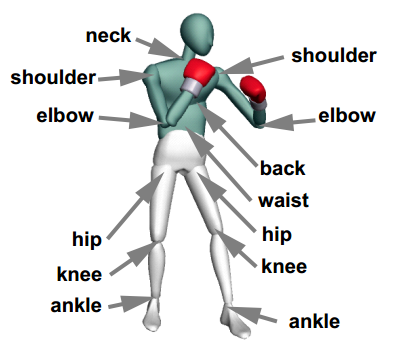
\includegraphics[height=150px]{artigos/2002_SCA_Motion_capture-driven_simulations_that_hit_and_react_p89-zordan/fig_model.png}
  \caption{Cada uma das juntas possui três graus de liberdade. Os valores de massa e parâmetros de inércia são calculados baseados nos modelos geométricos e nas medidas de densidade humana.}
  \label{fig:2002:mocap_sim:fig1}
\end{figure}

\subsubsection{Controle baseado em motion capture}

Os modelos utilizados, como dito anteriormente, são figuras humanas. Na figura \ref{fig:2002:mocap_sim:fig1} vemos os graus de liberdade do modelo humano utilizado para os experimentos. O nó raiz do movimento é considerado na pelvis. 
Para conseguir o controle dos movimentos capturados, um controlador de trajetória e um algoritmo que combina sequencias de movimentos capturados. O Torque de cada junta é calculado por um controlador "proporcional-derivado".

\begin{equation}
  \label{eq:2002:mocap:pdcontroller}
	\tau_t = k_t (\theta_d - \theta) - b_t (\dot{\theta})
\end{equation}

Assim como no artigo anterior. Agora é possivel o personagem seguir os dados de captura. 
Para tornar mais preciso, o sistema pode considerar o momento de inercia de toda a cadeia afetada pela junta, fazendo com que o número de parâmetros para ajustar as juntas do corpo sejam reduzidas, podendo ser até mesmo a mesma para todo o modelo, aumentando a velocidade e melhorando o desempenho do processo de ajuste.
Vale lembrar que sem o devido controle de feedback ou de interação com o ambiente, o personagem provavelmente iria cair sem fazer nada.

\subsubsection{Controle para bater}
Para criar animações que precisam de maior precisão e agilidade, como um soco, a técnica pura não pode ser utilizada. Para o exemplo do soco, foi feito um controle sobre o efetor final das mãos de forma que a animação atinja a posição desejada, e ajustando a escala de tempo para que a duração seja apropriada.
Primeiramente é utilizada uma solução de cinemática inversa para ajustar a posição do movimento bruto da captura. Isso permite novos movimentos que não estavam na biblioteca serem executados também.
Uma máquina de estados é adicionada para ter maior controle sobre a animação, como podemos ver na figura \ref{fig:2002:mocap_sim:fig2}.

\begin{figure}[ht]
  \centering
  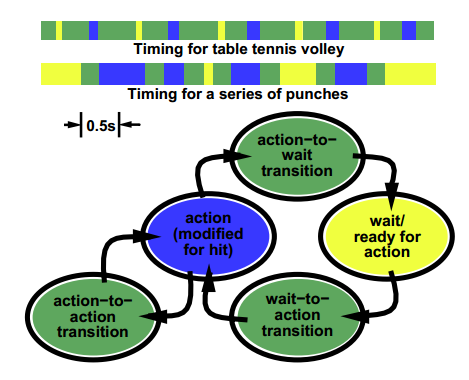
\includegraphics[height=150px]{artigos/2002_SCA_Motion_capture-driven_simulations_that_hit_and_react_p89-zordan/fig_state.png}
  \caption{Máquina de estados para o soco e para a cena da raquete. A cor das barras indica a duração de cada estado para cada uma das animações.}
  \label{fig:2002:mocap_sim:fig2}
\end{figure}

O final de um segmento de animação é interpolado com o segmento seguinte. Ações são enfileiradas para quando uma atividade chegar ao fim, a próxima iniciar.

\subsubsection{Reagindo a contatos}

O valor de ajuste, se muito alto, pode fazer com que a animação fique muito proxima da captura de movimento, e ignorando a simulação de impacto. Uma possibilidade é mudar o valor do ajuste de acordo com a ação que está acontecendo. Apenas os valores da região do corpo afetadas pelo movimento podem ser ajustadas, para dar o maior realismo possível para a animação.

\subsubsection{Equilibrando e rastreando}

A ideia do equilíbrio está relacionada ao centro de massa. Muitas ideias de controladores de equilibrio tentam minimizar a velocidade ou a aceleração do centro. A diferença dos problemas comuns para este é que a parte de baixo do corpo também está sob controle da captura de movimento.
Para conseguir o equilibrio, duas técnicas foram combinadas. Um "atuador virtual" calcula forças virtuais, e transforma elas em torques nas juntas, que representam o que o personagem pode fazer para se equilibrar com sua propria musculatura. Esse torque calculado é combinado com o torque da captura de movimento.
O intuito é manter o centro de massa proximo o suficiente de um centro de suporte, ponto simples de ser calculado baseado no polígono de apoio do personagem.

% ..........................................................
\subsubsection{Resultados}

Foram implementados diversos exemplos para ilustrar diversos aspectos do sistema.
No exemplo do tênis de mesa, o desafio era atingir uma bola em movimento a fim de mandá-la com uma determinada direção e velocidade. Portanto, a posição, orientação e velocidade da raquete precisam ser controladas.
No exemplo do boxe, considerado a maior contribuição do trabalho, foi a criação de um personagem a partir de dados de captura que podem interagir de maneira genérica. Animações de diferentes tipos de soco são modificadas utilizando cinemática inversa, fazendo com que o pugilista atinja posições epecíficas. Além disso, um personagem atinge o outro, sendo possível testar também a simulação de impacto, o equilíbrio e quanto o personagem consegue se manter proximo a sua simulação original.
No exemplo do personagem dançante, uma luva controlada pelo usuário pode interromper a animação com socos. Se a força for grande demais, o personagem pode até dar um passo involuntário para manter o equilíbrio. 

\begin{figure}[ht]
  \centering
  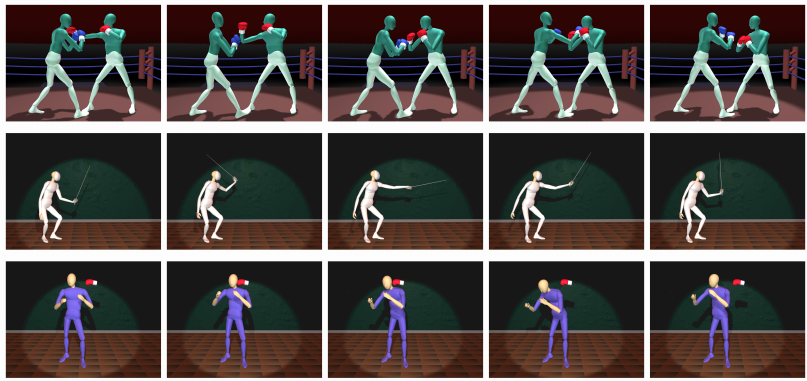
\includegraphics[height=150px]{artigos/2002_SCA_Motion_capture-driven_simulations_that_hit_and_react_p89-zordan/fig_examples.png}
  \caption{Exemplos para testar casos específicos de animação. Boxe, esgrima e um personagem dançando sendo atingido na cabeça.}
  \label{fig:2002:mocap_sim:fig3}
\end{figure}

% ============================================================================
\subsection{Pontos fortes} %no máximo três
\begin{itemize}
  \item Simulação combina mocap com restrições físicas para o corpo do personagem inteiro.
  \item Permite flexibilidade ao combinar com outras tecnicas de animação para permitir modificação dos dados brutos de captura.
\end{itemize}  

% ============================================================================
\subsection{Limitações} %no máximo três
\begin{itemize}
  \item A simulação em cima da captura de movimentos pode tornar a animação "suave", dificultando certas ações de acontecerem.
  \item A ideia de deixar mais automatico possivel se perde quando é preciso criar um grafo de controle de poses especiais.
\end{itemize} 


% ============================================================================
\subsection{Avaliação}
%\textbf{(a) Avanço considerável (\textit{Breakthrough}).}
 \textbf{(b) Contribuição significativa.}
% \textbf{(c) Contribuição modesta.}
% \textbf{(d) Contribuição fraca.}
% \textbf{(e) Sem contribuição.}
Muitos artigos semelhantes já existem na área. Porém é uma contribuição considerável visto o ganho de desempenho e o controle das ações mais detalhadas, através da máquina de estados.
Mas a parte mais significativa do artigo é a reação a impactos. A simulação resiste a diversos tipos de interações com os personagens, tentando manter a animação original na medida do possível, mas sem perder o realismo.

% ============================================================================
\subsection{Problema em aberto}
 \begin{itemize}
   \item Combinar simulação e animação de forma realmente automática. Muitos tipos de animação não podem ser obtidos a partir do dado bruto capturado, sendo necessária a interferência de um animador.
   \item O cálculo do impacto pode requerer mais precisão a medida que mais detalhes forem sendo adicionados à animação. O sistema atual funciona sob diversas restrições, como remoção de partes do corpo com pouca massa ou juntas desnecessárias para a animação a nível macroscópico.
 \end{itemize}  

% ============================================================================
\subsection{Aspecto obscuro}
 \begin{itemize}
   \item Não parece haver uma técnica para decidir quais aspectos implementar para cada animação. Parece que cada animação diferente requer uma adição à tecnica original para funcionar.
 \end{itemize}  

\chapter{Mês de outubro}

\section{\textit{Teaching a Robot to Grasp}}


% ============================================================================
\subsection{Referência completa do artigo}

\begin{itemize}
  \item \textbf{Autores:} Ludovic Hamon, Philippe Lucidarme, Paul Richard, Emmanuelle Richard
  \item \textbf{Local:} LISA Laboratory, University of Angers 62, France
  \item \textbf{\textit{Journal}:} Presence: Teleoperators and Virtual Environments [Qualis B2]
  \item \textbf{Data:} June 2011
  \item \textbf{Referência:} \citeonline{bib:2011:teaching-grasp}
\end{itemize}


% ============================================================================
\subsection{Resumo}
% ..........................................................
\subsubsection{Abstract}

Humans possess the ability to perform complex manipulations without the need to consciously perceive detailed motion plans. When a large number of trials and tests are required for techniques such as learning by imitation and programming by demonstration, the virtual reality approach provides an effective method. Indeed, virtual environments can be built economically and quickly and can be automatically re-initialised. In the fields of robotics and virtual reality, this has now become commonplace. Rather than imitating human actions, our focus is to develop an intuitive and interactive method based on user demonstrations to create humanlike, autonomous behaviour for a virtual character or robot. Initially, a virtual character is built via real-time virtual simulation in which the user demonstrates the task by controlling the virtual agent. The necessary data (position, speed etc.) to accomplish the task are acquired in a Cartesian space during the demonstration session. These data are then generalised off-line by using a neural network with a back-propagation algorithm. The objective is to model a function that represents the studied task, and by so doing, to adapt the agent to deal with new cases. In this study, the virtual agent is a six-degrees-of-freedom arm manipulator, Kuka Kr6, and the task is grasp a ball thrown into its workspace. Our approach is to find the minimum number of necessary demonstrations while maintaining an adequate task efficiency. Moreover, the relationship between the number of dimensions of the estimated function and, the number of human trials is studied depending on the evolution of the learning system.

% ..........................................................
\subsubsection{Propósito do artigo}
O artigo parece tratar o problema de programar uma máquina para realizar a tarefa de rastrear um objeto, e, de acordo com sua tarefa definida, alcançar ou se afastar daquele objeto. Então acredito que seja um bom ponto de partida para a pesquisa.

% ..........................................................
\subsubsection{Técnicas utilizadas} 
\begin{itemize}
  \item Redes Neurais
  \item Programming by demonstration
  \item Virtual Reality - Simulação virtual do ambiente
  \item Cinemática Inversa
  \item Motion Capture
  \item Haptic Feedback
\end{itemize} 

% ..........................................................
\subsubsection{Contribuição em relação a artigos anteriores} %mais ou menos 10 linhas
 \begin{itemize}
   \item A forma como utiliza a percepção e planejamento simplificado do ser humano e traduz para um ponto de captura da bola através do treinamento.
   \item A forma como a rede neural é utilizada. Foi feita uma generalização no espaço cartesiano do dado registrado pela demonstração humana. A demonstração cria uma função que permite o robô se adaptar a novos casos que não haviam sido demonstrados.
   \item Estudo do impacto da variação do número de dimensões em relação ao número necessário de demonstrações. Assim é possível determinar um número mínimo de demonstrações que mantenham o nível de performance da tarefa.
 \end{itemize}  

% ============================================================================
\subsection{Metodologia}
% Descreva um pouco mais detalhadamente a metodologia e os resultados do artigo. 
% Inclua as figuras que achar mais relevantes.

\subsubsection{Motivação}
	Seres humanos têm a capacidade de realizar tarefas simples melhor do que máquinas por causa da habilidade de realizar tarefas complexas sem a necessidade de conscientemente perceber todos os detalhes do movimento. Deste modo, o movimento humano pode ser utilizado para ensinar a máquina, usando a técnica de programação por demonstração.
	O problema é realizar diversas etapas do treinamento usando máquinas reais, pois o ambiente precisa ser remontado para dar inicio a uma nova iteração. Fazendo uso de um ambiente virtual é possível realizar diversas etapas do treinamento sem necessitar de um braço mecânico real, por exemplo. O objetivo do treinamento não é que o agente imite o comportamento humano, mas que ele consiga, ao final, realizar a tarefa de maneira autônoma.
	A tarefa definida para ser realizada é  a de um braço mecânico capturar uma bola arremessada. Esse braço deve ser treinado para alcançar a bola, e segurá-la.

\subsubsection{Conceitos Utilizados}
	Captura de objetos é uma tarefa que requer soluções em tempo real, processos e modelos que representem ações humanas. Por isso a primeira tarefa é resolver a quetão da intuitividade na interação humano-robô. Assim, é possível programar rapidamente e intuitivamente. 
Artigos anteriores justificam o uso da realidade virtual como ferramenta para encurtar e diminuir os custos do processo de aprendizagem, pois pode ser construido com preço bem mais acessível e rapidamente reinicializado.
	A quantidade de testes para treinar o ator podem exceder as centenas, e por conta disso uma restauração do ambiente inicial rápida é algo tão importante.
O sistema também pode criar casos de treino a partir de captura de movimento. Um banco com movimentos é criado, e mais movimentos podem ser criados a partir da interpolação de capturas existentes, os pseudo-exemplos. 

\subsubsection{Aplicação}
	A aplicação foi escrita em C/C++ e OpenGL. A simulação contém os seguintes objetos virtuais: Uma bola, uma mão controlada pelo usuário e um braço mecânico. A bola virtual é animada de acordo com a segunda lei de newton.
	
\begin{figure}[ht]
  \centering
  
\includegraphics[height=150px]{artigos/2011-Teaching_a_Robot_to_Grasp/fig1.png}
  \caption{A simulação virtual.}
  \label{fig:2011:teaching_grasp:fig1}
\end{figure}

	O braço mecânico é chamado de Kuka Kr6. Ele possui 6 eixos de rotação. A figura \ref{fig:2011:teaching_grasp:fig2} ilustra a topologia.
\begin{figure}[ht]
  \centering
  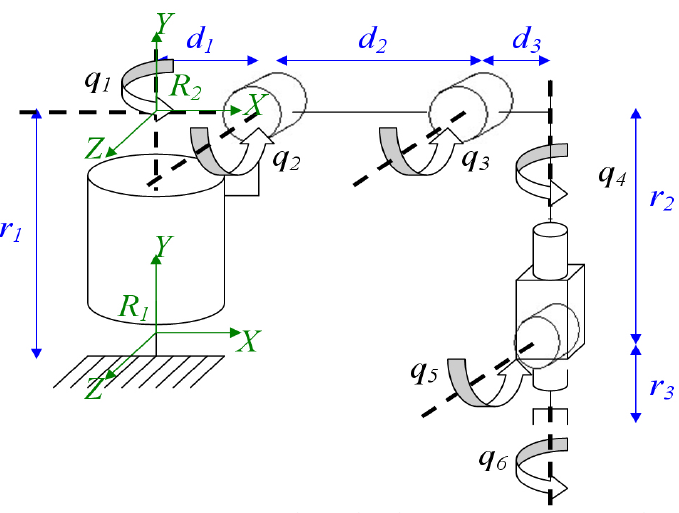
\includegraphics[height=150px]{artigos/2011-Teaching_a_Robot_to_Grasp/fig2.png}
  \caption{Parâmetros de construção do modelo de Kuka Kr6.}
  \label{fig:2011:teaching_grasp:fig2}
\end{figure}
	O agarrador tem uma posição cartesiana de acordo com os 6 ângulos dado pelo modelo geométrico direto definido por X=f(Q) onde X=(x,y,z) e Q=(q1,q2,q3,q4,q5,q6).
Para conseguir o valor dos 6 angulos de rotação, é usado a técnica geométrica inversa. Sem restrições, a área de atuação de Kuka Kr6 é definida por um torus.

\subsubsection{Interface de rastreio e captura do objeto}
	Usar um agente virtual como marionete em tempo real tem diversos problemas a respeito da área de trabalho. Como simular a restrição de movimento do braço do robô para o usuário? Uma possibilidade é o uso de interfaces hápticas.
	Isso pode ser um problema com grandes áreas de trabalho. Existem diversas técnicas para prover feedback háptico e produzir capturas de movimentos para humanos inteiros.
	Para a captura do objeto, é levantada a possibilidade do uso de luvas de RV. Porém o equipamento é frágil e ao ser usado diversas vezes para esse fim pode sofrer danos. Para contornar esse problema, outra técnica é utilizada onde uma esfera de colisão virtual é colocada no gripper do braço mecânico. A esfera tem um tamanho pre-definido e posicionada de acordo com o braço. Um mouse optico simples é utiilzado para comandar o fechamento ou abertura da mão, poupando o equipamento de captura.
\begin{figure}[ht]
  \centering
  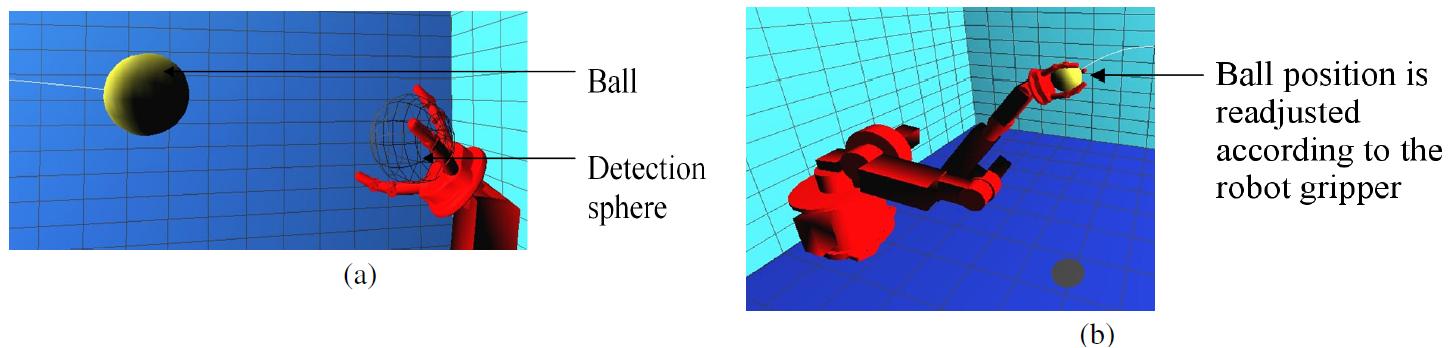
\includegraphics[width=250px]{artigos/2011-Teaching_a_Robot_to_Grasp/fig3.png}
  \caption{Sistema de grasping: (a) a esfera de colisão do grasp é renderizada apenas para visualização. (b) O centro do objeto colidiu com a esfera de colisão, e a sua posição foi reajustada para simular o grasp.}
  \label{fig:2011:teaching_grasp:fig3}
\end{figure}
	Para controlar o efetor final do robô, uma mão virtual é criada. A ideia é que a posição da mão virtual seja combinada com a posição da garra do robô. Em um dado quadro, é verificado se a mão do personagem virtual está numa posição pertencente a área de atuação do braço mecânico, e se isso acontecer, o braço é posicionado sobre a mão. O modelo geométrico inverso é utilizado para encontrar os ângulos do braço mecânico.

\subsubsection{Processo de aprendizado}
	O braço robô deve ser capaz de determinar a posição e a velocidade da bola em um determinado momento. Isso fará com que ele possa saber a trajetória da mesma, e se ela está em um espaço alcançável. Podem existir diversos pontos de encontro entre a área de atuação do braço mecâncio e a trajetória da bola.
	Para contornar o problema de definir o ponto de encontro, conhecido como “problema do encontro”, e prever a trajetória da bola, o usuário irá indicar onde o braço deve estar para agarrar a bola, toda vez que a bola é arremessada.
	Para simplificar e restringir o processo de aprendizado, algumas definições foram tomadas: A bola tem posição fixa, a trajetória é parabólica, a bola tem que passar pela área de atuação do braço mecânico. 
	Bolas são arremessadas em direção ao robô até que ele consiga agarrar 600 delas, controlado pelo humano. As bolas são jogadas com um vetor velocidade inicial aleatório.
\begin{figure}[ht]
  \centering
  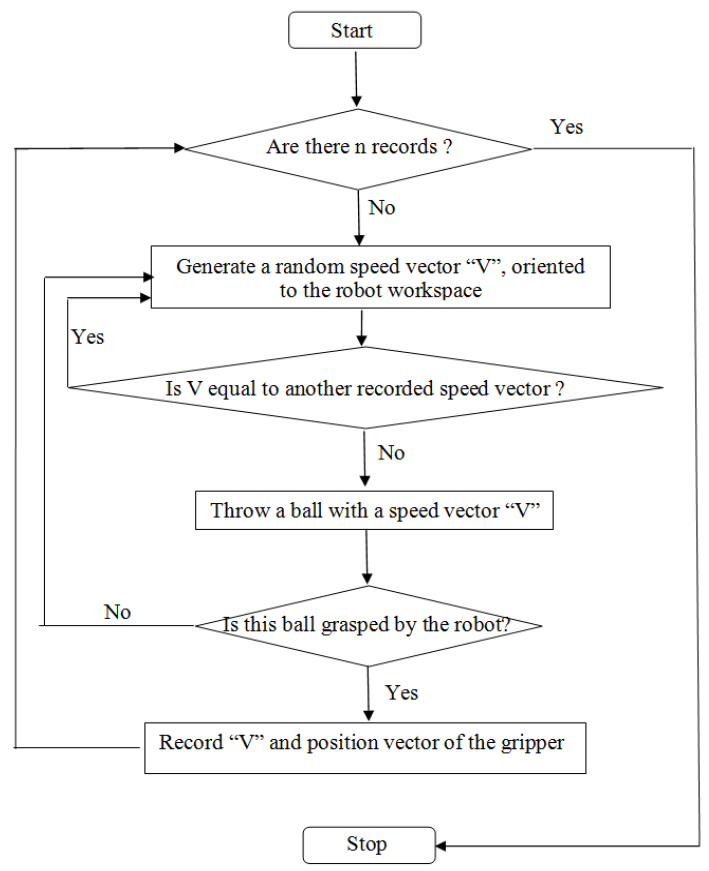
\includegraphics[height=200px]{artigos/2011-Teaching_a_Robot_to_Grasp/fig6.png}
  \caption{Diagrama do processo de demonstração. n é o número de demonstrações necessárias.}
  \label{fig:2011:teaching_grasp:fig6}
\end{figure}
	Para cada vetor de velocidade inicial, a posição da garra é registrada. O objetivo é construir uma rede neural que tenha como entrada o vetor velocidade, e como saída a posição da garra.
\begin{figure}[ht]
  \centering
  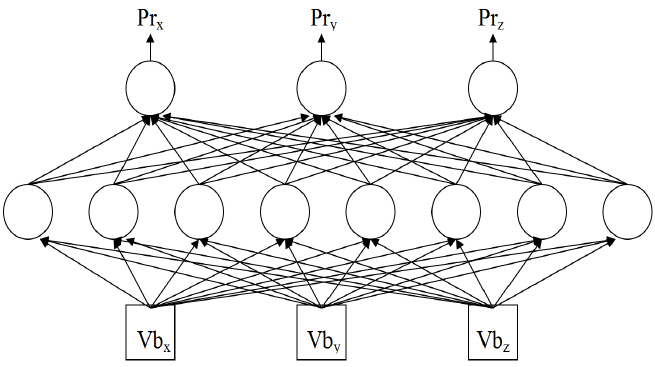
\includegraphics[height=150px]{artigos/2011-Teaching_a_Robot_to_Grasp/fig7.png}
  \caption{Diagrama da rede neural. O vetor de velocidade inicial serve de entrada, que passa por uma camada contendo 8 neurônios, e tem como saída em 3 neurônios finais as coordenadas do efetor final do braço.}
  \label{fig:2011:teaching_grasp:fig7}
\end{figure}
% ..........................................................
\subsubsection{Resultados}
A realidade virtual permitiu um aumento na eficiência da etapa de treino. Além disso, diversas medidas podem ser feitas mais facilmente a partir dos dados da simulação.

\begin{figure}[ht]
  \centering
  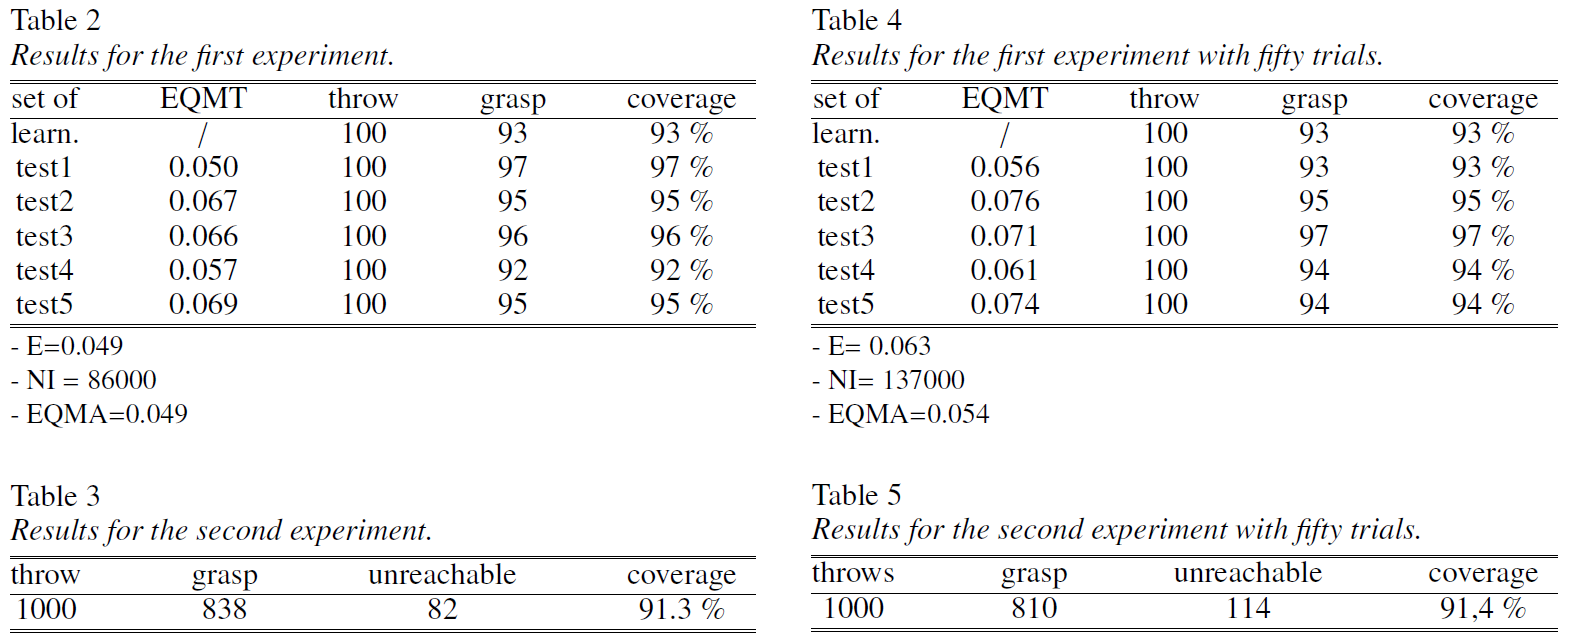
\includegraphics[width=300px]{artigos/2011-Teaching_a_Robot_to_Grasp/fig8.png}
  \caption{Tabelas contendo resultados para os experimentos.}
  \label{fig:2011:teaching_grasp:fig8}
\end{figure}

Experimento 1: Aprendizado. 100 arremessos foram realizados. A rede neural dá a posição que a garra deve atingir. O número de vezes que a garra captura a bola é contada e exibida na tabela 2. A porcentagem mostra que o agente se adaptou a novos casos, capturando mais do que durante a fase de treinamento.

Experimento 2: Eficiência. 1000 arremessos são feitos com um vetor velocidade aleatório. O numero de capturas do objeto e o numero de perdas é contado. É verificado se há vetores repetidos entre os gerados aleatoriamente. Com cobertura de mais do que 90%, o resultado é consistente com o do primeiro experimento. O agente adquiriu comportamento autônomos das demonstrações humanas com nível aceitável de eficácia.


% ============================================================================
\subsection{Pontos fortes} %no máximo três
\begin{itemize}
  \item O algoritmo proposto converge com  um numero relativamente pequeno de inputs de humanos.
  \item Demonstra um nível aceitável de eficiência.
\end{itemize}  

% ============================================================================
\subsection{Limitações} %no máximo três
\begin{itemize}
  \item Precisa da interação humana
  \item Não utiliza visão (o input da rede é um vetor velocidade). Seria preciso estimar essa velocidade com uma rede neural para dar certo.
\end{itemize} 


% ============================================================================
\subsection{Avaliação}
%\textbf{(a) Avanço considerável (\textit{Breakthrough}).}
% \textbf{(b) Contribuição significativa.}
 \textbf{(c) Contribuição modesta.}
% \textbf{(d) Contribuição fraca.}
% \textbf{(e) Sem contribuição.}
Existem outros artigos semelhantes que trazem resultados muito bons também. Foi uma boa tentativa de simplificar o processo e focar na parte da aprendizagem. Para mim, o artigo foi importante pois introduziu a ideia do uso de rede neural para treino por demonstração.

% ============================================================================
\subsection{Problema em aberto}
 \begin{itemize}
   \item Primeira extensão desse trabalho seria determinar o número mínimo de tentativas para atingir um determinado grau de eficiência. Isso requer mais estudos, mais testes e dependem das restrições e dos resultados esperados.
 \end{itemize}
\section{\textit{A Multiple Hypothesis Approach
for a Ball Tracking System}}


% ============================================================================
\subsection{Referência completa do artigo}

\begin{itemize}
  \item \textbf{Autores:} Oliver Birbach and Udo Frese
  \item \textbf{Local:} Bremen, Germany
  \item \textbf{\textit{Journal}:} International Conference on Computer Vision Systems [Qualis ??]
  \item \textbf{Data:} 2009
  \item \textbf{Referência:} \citeonline{bib:2009:multiple-hypothesis}
\end{itemize}


% ============================================================================
\subsection{Resumo}

\subsubsection{Abstract}
This paper presents a computer vision system for tracking
and predicting flying balls in 3-D from a stereo-camera. It pursues a “textbook-style” approach with a robust circle detector and probabilis tic models for ball motion and circle detection handled by state-of-theart estimation algorithms. In particular we use a Multiple-Hypotheses Tracker (MHT) with an Unscented Kalman Filter (UKF) for each track, handling multiple flying balls, missing and false detections and track
initiation and termination. The system also performs auto-calibration estimating physical parameters (ball radius, gravity relative to camera, air drag) simply from observing some flying balls. This reduces the setup time in a new environment.

% ..........................................................
\subsubsection{Propósito do artigo}
A ideia era encontrar um artigo que pudesse rastrear algum tipo de objeto usando câmera. Esse artigo de fato faz isso, porém ele utiliza técnicas probabilísticas e processamento de imagens para detectar apenas círculos na tela, e com isso, poder rastrear. Nesse caso, toda a matemática do problema teve de ser pensada para elaborar um algoritmo específico para um tipo de objeto em um tipo de comportamento. Não era bem o que eu estava procurando. Farei, de modo resumido, a leitura.

% ..........................................................
%\subsubsection{Técnicas utilizadas} 
% \begin{itemize}
%   \item xxx
% \end{itemize}  
%xxx

% ..........................................................
%\subsubsection{Contribuição em relação a artigos anteriores} %mais ou menos 10 linhas
% \begin{itemize}
%   \item xxx
% \end{itemize}  
%xxx

% ============================================================================
\subsection{Metodologia}


	Inicialmente o artigo descreve a disposição do sistema de captura. Duas cameras capturam imagem de uma mesma cena. Um detector de círculos identifica os artefatos nas imagens capturadas. Os círculos identificados são colocados em um rastreador, que aplica um método estatístico para obter a posição e a velocidade de cada uma das bolas.
	A forma que a detecção de círculo funciona é simples: Ele identifica um provável píxel de círculo, fazendo uma busca exaustiva na imagem, procurando por bordas. Ao encontrar uma borda, percorre no sentido perpendicular à tangente da superficie, esperando encontrar o raio. Como o raio é possível estimar a distância da bola para o observador, considerando que o raio da bola seja previamente conhecido.
	Então ele define o Single Track Probabilistic Model, que prevê o movimento da bola, ou seja, posição e velocidade, a partir das imagens capturadas. O modelo é baseado nas fórmulas classicas da mecânica, que incluem gravidade e atrito do ar.  Para estimar a distância da bola, o seu diâmetro é levando em consideração. Portanto o método se restringe a um tamanho conhecido de bola.
	Utilizar o método anterior para associar todas as medidas realizadas a diversas bolas é uma tarefa dificil. Alguns artefatos podem estar oclusos por outros, ou aparecendo em determinado quadro e em outro não. Alarmes falsos como a cabeça de uma pessoa também precisa ser eliminada do processo de rastreio. Para cada trilha rastreada, é associada uma probabilidade de ser um falso alarme. Para cada hipotese m e tempo k, ele calcula a probabilidade.
	Quando está utilizando imagens estereoscópicas, ou seja, duas câmeras, é preciso fazer uma associação entre os objetos que aparecem em uma imagem com os da outra imagem. Nesse caso, utilizando o método proposto, ele poderia combinar os elementos das duas imagens antes de tentar rastrear e integrar os resultados como um valor 3D. A segunda opção é deixar o método implicitamente gerenciar essa questão dos candidatos a serem o mesmo objeto.
	É importante lembrar dos parâmetros utilizados na fórmula, que incluem a gravidade, o diâmetro da bola, e a calibração das câmeras (distância de uma para a outra por exemplo).  Os parâmetros são estimados com objetos sendo arremessados durante a fase de calibragem.

 ..........................................................
\subsubsection{Resultados}
A detecção de círculo usada é comparada com o OpenCV. Ele sugere que a implementação que fizeram para essa aplicação em particular pode ser mais robusta.
Como resultado, foi apresentado uma solução para rastreio de múltiplas bolas a partir de uma câmera estática. O algoritmo não possui quase nenhuma heurística ou parâmetros de ajuste na detecção do círculo.

% ============================================================================
\subsection{Pontos fortes} %no máximo três
\begin{itemize}
  \item Algoritmo robusto de detecção de círculos
  \item Apesar das restrições de uso, parece fazer bem tudo que se propôs a fazer.
\end{itemize}  

% ============================================================================
\subsection{Limitações} %no máximo três
\begin{itemize}
  \item Restrições quanto ao posicionamento da câmera e movimentação da mesma.
  \item Método muito limitado ao problema de detecção e rastreio de esferas. Parece uma técnica difícil de generalizar.
\end{itemize} 


% ============================================================================
%\subsection{Avaliação}
%\textbf{(a) Avanço considerável (\textit{Breakthrough}).}
% \textbf{(b) Contribuição significativa.}
 \textbf{(c) Contribuição modesta.}
% \textbf{(d) Contribuição fraca.}
% \textbf{(e) Sem contribuição.}
%Justificativa.

Apesar do artigo parecer ter uma contribuição significativa para a sua respectiva área, para o meu trabalho parece ter servido apenas como uma forma de podar a árvore de busca de assuntos. No momento não pretendo utilizar um modelo matemático ou estatístico fixo para um tipo de objetos. Atualmente é interessante um sistema que possa ser treinado/programado para casos mais gerais.

% ============================================================================
\subsection{Problema em aberto}
 \begin{itemize}
   \item Possibilitar acoplar a câmera em um capacete ou utilizar um HMD.
   \item Pular ou combinar etapas do processo para otimizar e melhorar desempenho.
 \end{itemize}  

% ============================================================================
%\subsection{Aspecto obscuro}
% \begin{itemize}
%   \item xxx
% \end{itemize}  
%xxx
\section{\textit{A VISION-BASED APPROACH TO
BEHAVIORAL ANIMATION}}


% ============================================================================
\subsection{Referência completa do artigo}

\begin{itemize}
  \item \textbf{Autores:} Olivier Renault and Nadia Magnenat-Thalmann and Daniel Thalmann
  \item \textbf{Local:} Computer Graphics Lab, Swiss federal Institute of Technology
  \item \textbf{\textit{Journal}:} The Journal of Visualization and Computer Animation [Qualis ??]
  \item \textbf{Data:} 20 JUL 2011
  \item \textbf{Referência:} \citeonline{bib:2011:vision-based}
\end{itemize}


% ============================================================================
\subsection{Resumo}
% ..........................................................
\subsubsection{Abstract}
This paper presents an innovative way of animating actors at a high level based on the concept of synthetic vision. The objective is simple: to create an animation involving a synthetic actor automatically moving in a corridor avoiding objects and other synthetic actors. To simulate this behaviour, each synthetic actor uses a synthetic vision as its perception of the world and so as the unique input to its behavioural model. This model is based on the concept of Displacement Local Automata (DLA), which is similar to the concept of a script for natural language processing. A DLA is an algorithm that can deal with a specific environment. Two DLA's are described in detail called follow-the-corridor and avoid-the-obstacle.

% ..........................................................
\subsubsection{Propósito do artigo}
O artigo utiliza o conceito de visão para definir um comportamento evasivo ao ator. Isso lembra um pouco o que estou buscando.

% ============================================================================
\subsection{Metodologia}
% Descreva um pouco mais detalhadamente a metodologia e os resultados do artigo. 
% Inclua as figuras que achar mais relevantes.

O artigo define como funciona o sistema de captura de imagem. Diferente de sistemas robóticos onde há um processamento pesado na imagem para extrair informações como profundidade ou distância de objetos, o sistema proposto pega um atalho usando como vantagem as informações que já existem no sistema computacional virtual do ambiente. Porém, essa informação não pode ser obtida de qualquer maneira. É preciso limitar as informações ao campo visual do personagem, pois além de melhorar o desempenho no caso de uma cena muito complexa, aumenta o grau de realismo onde o personagem só percebe visualmente aquilo que está em seu campo de visão, e só então toma alguma ação.
As informações adicionais, além da imagem 2D da cena capturada pelo personagem, contém informação de distância, obtida através do z-buffer do algoritmo de renderização, e uma flag identificando a qual objeto aquele pixel pintado originalmente pertence.
Com essas informações, ele alimenta um controlador. Existem duas abordagens de controle: Em uma, para cada automato de controle, é enviada a condição de ativação extraida do input visual. Se positivo, ele executa sua ação. Um controlador não está ciente do outro. Isso pode causar conflitos e cada controlador precisa ter essa informação de quando deve ser ativado. A segunda opção é centralizar esta decisão e ativar o controlador mais adequado para cada situação.
Para este trabalho foram implementados dois automatos de controle, conhecidos como DLA's ou Displacement Local Automata. No primeiro, o comportamento de andar para frente em direção a saida do corredor. No segundo, um controle de desvio de obstáculos.
Desta forma, o personagem alterna seus comportamentos a fim de realizar a tarefa.

% ============================================================================
\subsection{Pontos fortes} %no máximo três
\begin{itemize}
  \item É um algoritmo bem simples, não faz uso de matemática complexa.
  \item Parece relativamente fácil de programar um comportamento bem específico, sendo possível programar caso a caso.
\end{itemize}  

% ============================================================================
\subsection{Limitações} %no máximo três
\begin{itemize}
  \item Não é uma solução muito genérica
  \item Não parece ter muita naturalidade na escolha dos movimentos. A unica preocupação do algoritmo é respeitar as restrições impostas.
\end{itemize} 


% ============================================================================
\subsection{Avaliação}
%\textbf{(a) Avanço considerável (\textit{Breakthrough}).}
% \textbf{(b) Contribuição significativa.}
% \textbf{(c) Contribuição modesta.}
 \textbf{(d) Contribuição fraca.}
% \textbf{(e) Sem contribuição.}

Parece um artigo interessante, mas sinto que a questão da visão utilizada por ele aborda um problema menos genérico. Ele trata para cada caso o imput visual para tomar uma decisão.

 
% \chapter{Mês de novembro}

\bibliography{bib}

\end{document}
